\documentclass[tikz,border=4pt]{standalone}
\usepackage{amsmath}
\begin{document}
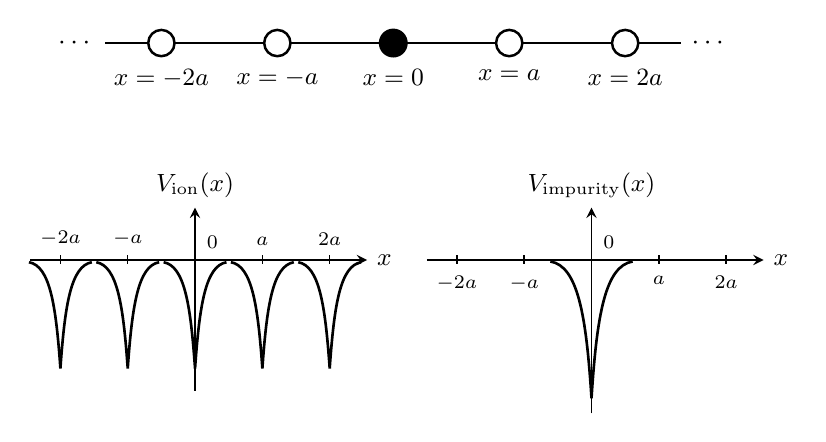
\begin{tikzpicture}[>=stealth, thick, scale=0.95]
  % Top: 1D lattice chain
  \begin{scope}[yshift=2.9cm]
    \draw[line width=0.8pt] (-3.85, 0) -- (3.85, 0);
    \node[left] at (-3.85, 0) {$\cdots$};
    \node[right] at (3.85, 0) {$\cdots$};
    \foreach \x/\lbl in {-3.1/-2a, -1.55/-a, 1.55/a, 3.1/2a} {
      \fill[white] (\x, 0) circle (5pt);
      \draw[line width=0.9pt] (\x, 0) circle (5pt);
      \node[below, font=\small] at (\x, -0.22) {$x = \lbl$};
    }
    \fill (0, 0) circle (5.5pt);
    \node[below, font=\small] at (0, -0.22) {$x = 0$};
  \end{scope}

  % Bottom-left: V_ion(x)
  \begin{scope}[xshift=-2.65cm, yshift=0cm]
    \draw[->, line width=0.65pt] (-2.2, 0) -- (2.3, 0) node[right, font=\small] {$x$};
    \draw[->, line width=0.65pt] (0, -1.75) -- (0, 0.7) node[above, font=\small] {$V_{\mathrm{ion}}(x)$};
    \node[above right, font=\scriptsize] at (0.02, 0.02) {$0$};
    \foreach \xc/\lbl in {-1.8/-2a, -0.9/-a, 0.9/a, 1.8/2a} {
      \draw[line width=0.5pt] (\xc, 0.06) -- (\xc, -0.06);
      \node[above, font=\scriptsize] at (\xc, 0.05) {$\lbl$};
    }
    % Periodic attractive wells centered at -1.8, -0.9, 0, 0.9, 1.8
    \foreach \xc in {-1.8, -0.9, 0, 0.9, 1.8} {
      \draw[line width=0.95pt] (\xc-0.42, -0.03) .. controls (\xc-0.14, -0.08) and (\xc-0.06, -0.6) .. (\xc, -1.45)
        .. controls (\xc+0.06, -0.6) and (\xc+0.14, -0.08) .. (\xc+0.42, -0.03);
    }
  \end{scope}

  % Bottom-right: V_impurity(x) (Delta V(x) schematic)
  \begin{scope}[xshift=2.65cm, yshift=0cm]
    \draw[->, line width=0.65pt] (-2.2, 0) -- (2.3, 0) node[right, font=\small] {$x$};
    \draw[->, line width=0.65pt] (0, -2.05) -- (0, 0.7) node[above, font=\small] {$V_{\mathrm{impurity}}(x)$};
    \node[above right, font=\scriptsize] at (0.02, 0.02) {$0$};
    \foreach \xc/\lbl in {-1.8/-2a, -0.9/-a, 0.9/a, 1.8/2a} {
      \draw[line width=0.5pt] (\xc, 0.06) -- (\xc, -0.06);
      \node[below, font=\scriptsize] at (\xc, -0.08) {$\lbl$};
    }
    \draw[line width=0.95pt] (-0.55, -0.02) .. controls (-0.18, -0.08) and (-0.07, -0.75) .. (0, -1.85)
      .. controls (0.07, -0.75) and (0.18, -0.08) .. (0.55, -0.02);
  \end{scope}
\end{tikzpicture}
\end{document}
